\documentclass{article}
\usepackage[english]{babel}
\usepackage[letterpaper,top=2cm,bottom=2cm,left=3cm,right=3cm,marginparwidth=1.75cm]{geometry}
\usepackage{amsmath}
\usepackage{setspace}
\usepackage[colorlinks=true, allcolors=blue]{hyperref}
\usepackage{graphicx}
\usepackage{listings}
\usepackage{subcaption}
\lstdefinestyle{racket-source-code}{basicstyle=\ttfamily\tiny}
\UseRawInputEncoding 

\title{\uppercase{Fitting Regimes into L1 cache}}
\author{Zane Enders & Professor Panchekha}
\date{\today}

\doublespacing
\begin{document}


\begin{titlepage}
    \begin{center}
    

       \vspace*{1cm}

        \textbf{\uppercase{Refactoring Regimes}}

       \vspace{0.5cm}
       
       \text{Zane Enders \& Pavel Panchekha}
       
       \date{\today}
            
       \vspace{1.5cm}

   
        A Senior Thesis Submitted to the Faculty of 
        The University of Utah
        In Partial Fulfillment of the Requirements for the
        Degree of Bachelor of Science
        In
        Computer Science
            
       \vspace{0.8cm}
            
       \vfill
    \end{center}
\end{titlepage}
\newpage

\pagenumbering{arabic}

\section{Abstract}
Herbie \cite{Herbie} is a compiler developed in collaboration between the University of Utah and the University of Washington that uses a rule-based AI technique to improve floating-point accuracy and execution speed for arbitrary mathematical expressions. Floating-point arithmetic is used widely across the industry in fields from numerics to popular large language models. The majority of the CPU and GPU are devoted to floating-point computation. We targeted a bottleneck in the Herbie pipeline in a phase called “regimes” and reduced its runtime by 3.5x and its memory usage by 7x.

\section{Introduction}
% TODO Rework this and maybe the intro
This paper explores the optimization of the Regimes phase within Herbie, a compiler for improving the accuracy of floating-point programs by providing alternative options for a given math expression. Herbie takes in a mathematical expression in the form of a specification as input and translates that into a representation, such as floating-point, then applies several phases to generate alternative expressions that may minimize rounding errors.

The Regimes phase plays a crucial role in Herbie's optimization process. It combines multiple alternative program representations generated from the original expression, aiming to create a more accurate final program. However, for some inputs, the original recursive Regimes algorithm wasn’t as performant as it could be and is relatively memory-intensive.

This paper introduces a new, iterative approach to the Regimes phase, that significantly improves the performance and memory usage. This optimization translates to a faster overall runtime for Herbie's nightly benchmark suite.

We will use the example $sqrt(x + 1) - sqrt(x)$, which is the default example in Herbie, pulled from Richards Hamming’s numerical textbook \cite{Hamming}. This example will show how Herbie improves the error in this expression. Visualized in Figure I (below) this example has high error for large positive inputs, which can be improved using Herbie.

\begin{figure}[ht]
\centering
\begin{minipage}{0.6\textwidth}
  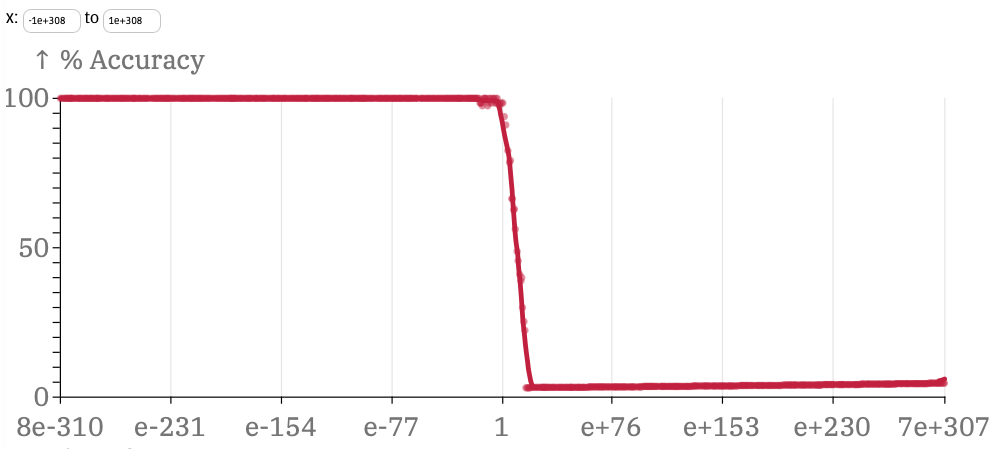
\includegraphics[width=\textwidth]{accuracy-graph.png}
\end{minipage}
\caption{\%Accuracy graph of the output $sqrt(x + 1) - sqrt(x)$.}
\label{fig:hypot-error-graph}
\end{figure}

\subsection{Herbie overview}

Herbie takes in a specification defined using Math expressions in the Real domain and then compiles them to an output representation that computers can work with, most commonly floating-point. Herbie uses a rules-based AI method that allows for the automated generation of suggestions of alternative ways of representing the input program that may be more accurate than the original. When combined with frontends like Odyssey \cite{Odyssey}, additional information may be surfaced, such as where the error in a given expression may be. Herbie uses quite a few terms that have a precise meaning. To help with clarity we define the following terms.

\subsubsection{Specifications}
A Specification allows for a source of truth to be defined for a given program. You can think of the source code passed to a compiler or interpreter as a specification of what the output program should produce. Defining this Specification allows Herbie to find different alternative ways of expressing the specification and measure how well this alternative is compared to the specification. Where a good solution to the Specification provides an accurate answer on all points.

\subsubsection{Programs \& Alternatives}
In Herbie programs are an instantiation of a specification with respect to a representation, like floating-point. The program instantiated from the original specification is used to get a metric of how accurate the program is compared to what's expected from its specification. This evaluation is done over the sampling and localization phases of Herbie (explained later). Different versions of the specification’s program are referred to as alternatives. These later materialize as Herbie’s output and can be converted to source code like what is shown in Figure \ref{fig:python}.

\subsubsection{Expressions}
Herbie operates on Specifications and their associated Programs, which are composed of mathematical expressions. These expressions and inherent sub-expressions are simply the operations, variables like $x$, or literals like $1$, of which the Specification and Programs are composed of. The example \newline $sqrt(x + 1) - sqrt(x)$ has seven sub-expressions, one for each Math operation. Numeric literals like $1/3$ are expressed as expressions because they can have an inherent error in them.

\subsubsection{Representation}
A representation is the numerical system that is being used by Herbie to represent the Real numbers. This is defined as a part of the specification. The most common representation used by Herbie is double-precision floating-point, and although there exist other representations, this is the representation that will be used throughout this paper.

\subsection{How Herbie Works}
Herbie first compiles a Specification like $sqrt(x + 1) - sqrt(x)$ to a program using a defined representation like floating-point which is used to evaluate the accuracy of this naive translation compared to what the correct answer is. This is done by sampling various inputs and outputs in the specification along with its associated program.

\subsubsection{Sampling}

To get a measure of how accurate a given program is compared to its Specification and to provide a target for Herbie to aim for. Herbie samples 8,256 uniformly distributed points from the domain of the program. If no subdomain is provided, the representation’s domain is used; in the case of floating-point, positive to negative infinity is used.

The program is then run with these sampled points to obtain their output and then compared against the specification. The correct answer for a given point is computed using Rival \cite{Rival}, which uses interval arithmetic and the library MPRF \cite{MPFR} to determine the correctly rounded answer for a program. The delta between the output of the program and the output of the specification gives a measure of how accurate a program is on a given point and is averaged together to approximate how accurate a program is compared to its specification. 

Now that Herbie has a correct answer and the answer provided by the initial program, Herbie can locate where in the program the error is likely occurring and will attempt to generate an alternative program that will be more accurate. The program’s average error over the entire input range serves as an approximation for how accurate a given program will be in real-world scenarios. This moves us into Herbie’s Main loop, which is shown in Figure \ref{fig:herbie-pipeline}.

\begin{figure}[htbp]
\begin{center}
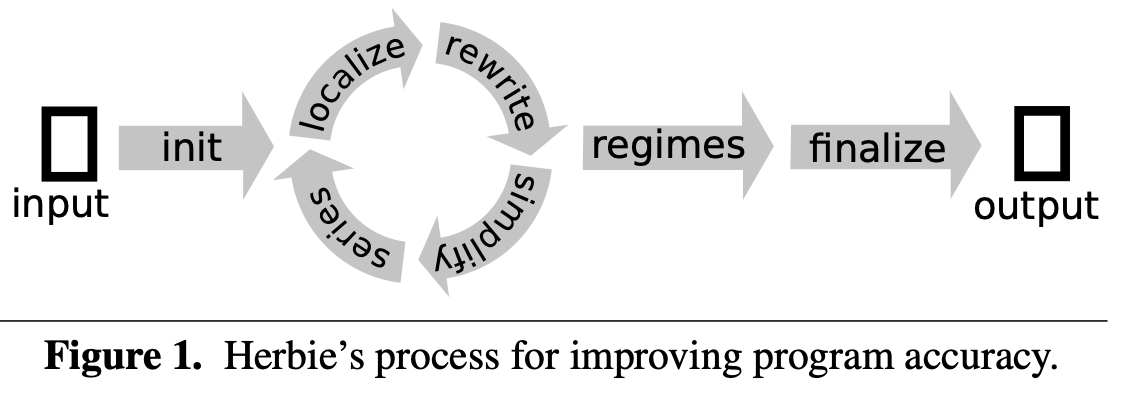
\includegraphics[scale=0.5]{herbie-pipeline.png}
\caption{Herbie's pipeline.}
\label{fig:herbie-pipeline}
\end{center}
\end{figure}

\subsection{Main Loop}
Herbie’s main loop is run multiple times and is used to generate alternatives for the original program using the sampled points and other properties that can be defined in the specification but are left out of this paper as they aren’t relevant to the topic of this paper. The first phase of the main loop is the Localize phase.

\subsubsection{Localize Phase}

The Localize phase is used to find which sub-expressions in the specification are likely to be responsible for the error. These expressions are where Herbie focuses on making improvements. In our \newline $sqrt(x + 1) - sqrt(x)$ example, the main cause of error is located in the subtraction operation because of what is called catastrophic cancellation. This is when the left and right-hand sides of the operation are very close to each other, and the majority of the remaining value is lost in rounding error. 

\subsubsection{Rewrite Phase}

The second phase of Herbie is to generate alternative programs for the original program. An “alternative program” is a possible variation of the original program that results from rewriting a sub-expression of the original program to a permutation of that expression using algebraic rewrite rules. This rewriting process is done using an eGraph\cite{eGraphs} which takes in as input a starting state and a set of possible transitions and produces a collection of possible ending states.

What’s considered a good and bad rewrite depends on what metric Herbie is focused on. For the purposes of this paper, Herbie is primarily focused on accuracy, however, other metrics could also be designed. These alternatives are then ordered and ranked. The worst alternatives are then pruned based on whether there is a more accurate alternative for a given point or if its average error is the highest of the set.

\subsubsection{Simplify Phase}
The third phase of the Herbie pipeline is to simplify the output expressions using a subset of the rewrite rules to remove unhelpful rewrites, such as repeatedly adding one to an expression when adding a different constant once would be better. This cleans up the output from the Rewrite phase.

\subsubsection{Series Phase}
The last part of the main loop is the Series phase. The Series phase performs a Taylor series expansion on sub-expressions since that form of the expansion could be more accurate than the original expression. This helps explore options that can not be explored by rewriting but could provide a more accurate approximation of a given expression.

After the main loop completes its iterations over the previous four phases to generate possible good alternatives, the alternatives are passed along to the Regimes phase of the compiler.

\subsection{Regimes Phase}

The regimes phase uses a dynamic algorithm that takes in alternatives generated in the main loop and potentially joins multiple alternatives together to produce new alternatives. Two programs are joined together by branching between them when an input falls into a certain subdomain of the specification domain. Figure \ref{fig:python} shows a code example of two programs branched together by Regimes to form a new program. Alternatives are combined based on their error at different regions of the input domain. From there the alternatives are passed to the finalize phase.

\begin{figure}[htbp]
\begin{center}
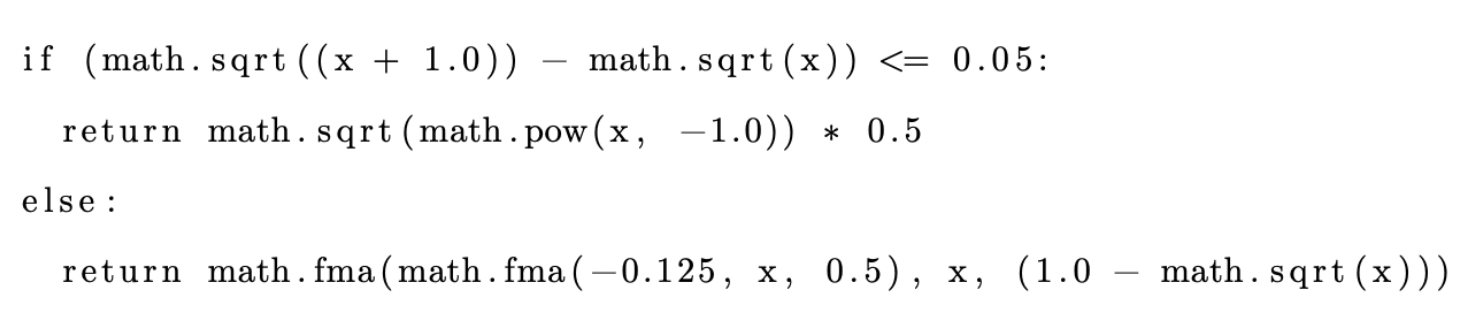
\includegraphics[scale=0.60]{python-regime.png}
\caption{A visualization of a split point.}
\label{fig:python}
\end{center}
\end{figure}

\subsection{Finalize Phase}
The Finalize phase of Herbie is where the generated set of alternatives is cleaned and the result is provided to the consumer of Herbie. The best re-write of our example is the expression $\frac{1}{\sqrt{x} + \sqrt{1 + x}}$, which nearly doubles the original accuracy by removing the subtraction operation.

This completes a very high-level summary of Herbie and allows us to move into the core of the paper which discusses speeding up the Regimes phase after the main loop.

\section{Methods}
The Regimes algorithm evaluates alternatives from the main loop based on their cumulative error, sampled over 256 points from the original set of sampled points. This cumulative error gives a uniform approximation of how good an alternative is vs the input space. The goal of the Regimes phase is to minimize this curve by using alternatives to generate a more accurate program. This is done by joining multiple alternatives where one performs best in one section and where another alternative performs poorly.  A possible regime output program is shown in the Python code in Figure \ref{fig:python}. These alternatives are joined together using a list of split points.

\subsubsection{Split Points}

\begin{figure}[htbp]
\begin{center}

\includegraphics[scale=0.60]{split-point.png}
\caption{A visualization of a split point.}
\label{fig:split-point}
\end{center}
\end{figure}

Split points define where to use one alternative vs another. A split point encodes when to branch between two given alternative programs. A split point is composed of an index that references the alternative that is being used and a threshold that defines the point before which the current alternative is to be used. These split points are later evaluated to generate a program in an output representation by branching between different alternatives as we move from left to right across the input range from negative infinity to positive infinity.

Any program can be expressed as a list of split points. For example, let’s say the first alternative in our input is the most accurate on all points and cannot be improved on. This could be represented as one split point for alternative 0 and point 256 as shown in Figure \ref{fig:split-point}. This says to use the alternative at index 0 for all points up to 256 or, in other words, don’t branch at all and just use the alternative at index 0. A list of only one Split Point means using that alternative for all points before that point. Associated with the list of alternatives is a list of booleans for each point that represents whether or not we can split at that point. This is used to avoid introducing split points when the value between two adjacent points is the same.

\subsubsection{Penalty value}

To avoid overfitting and using too many Split Points between alternatives for a given run, Regimes uses a penalty value. This penalty value is applied to the cumulative error of an alternative to favor or discourage adding split points. The Regimes algorithm works to minimize the cumulative error, so expressing the penalty in this way allows the algorithm to treat Split Points as having a cost. This penalty value helps avoid overfitting and adding a split point at each possible split point. Currently, this value is set to the total number of possible split points that could be made (256).

\subsection{Original Regimes Algorithm}
The original Regimes algorithm starts by mapping over the alternatives and generating a cumulative sum for each alternative. Recording the current cumulative error at each of the 256 possible split points. This cumulative error view of the alternatives is then used to generate a Candidate for each of these points. The Candidate at the last point represents our final output and its list of split points will be used to generate a new alternative.

A Candidate encapsulates the list of split points (in reverse order) and the cumulative error of those split points. The cumulative error can be found by adding up the error of each alternative for the error of the points it is being used for. Saving this sum allows for a quick comparison to determine if one Candidate is more accurate on average than another for the given set of points they represent. 

Below in Figure \ref{fig:candidate} is a candidate which represents the 5th candidate from Figure \ref{fig:candidate-list}.

\begin{figure}[htbp]
\begin{center}
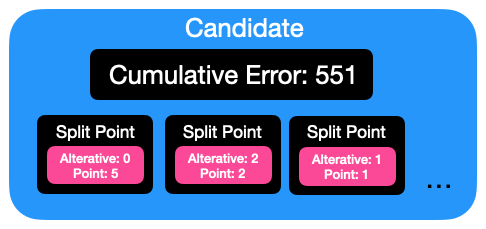
\includegraphics[scale=0.69]{candidate.png}
\caption{A visualization of a Candidate.}
\label{fig:candidate}
\end{center}
\end{figure}

A Candidate is generated for each point by creating a split point for the alternative with the lowest cumulative error at that point and recording that error. This results in 256 Candidates all with one split point for the alternative that had the lowest cumulative error at that point. These Candidates are then optimized as sub-problems in the core loop of the algorithm

\begin{figure}[htbp]
\begin{center}
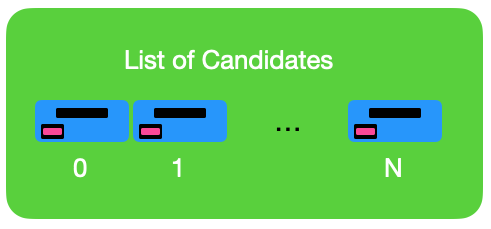
\includegraphics[scale=0.69]{list-of-candidates.png}
\caption{A visualization of a list of Candidates.}
\label{fig:list-of-candidates}
\end{center}
\end{figure}

This list of 256 Candidates is passed to a function called “add split point” which optimizes each candidate as a sub-problem by using the Candidates that represent the points before it to construct a potential better Candidate for that point. This is done by looping over each of the previous Candidates and then looping over all alternatives and finding the alternative with the lowest cumulative error between the previous Candidate’s point and the point we are currently optimizing, a value that will be referred to as the “error delta.” This error delta is added to the error of the candidate that represents a potential new candidate for the point being optimized. We compare this potential candidate with the current candidate (possibly the initial candidate selected) and see if the new candidate has a lower error than the current candidate. We favor the current candidate by subtracting our penalty value from its cumulative error. If the new Candidate’s error is less than this favored value we replace the current Candidate with the new Candidate by taking the list of Candidates from a previous candidate and appending a split point for the point that the candidate represents and setting its alternative index to the alternative we used which had the lowest delta increase in error.

The “add split point” function returns a new list of Candidates which is then compared to its input list of Candidates to determine if any changes occurred. If there were changes, we apply the algorithm again to the new list of Candidates. This is repeated until no changes occur between recursive calls, which indicates that no more split points can be added to reduce the cumulative error for any of the Candidates and their associated subproblems. A toy visualization of this ending list of Candidates is shown in Figure \ref{fig:candidate-list} which has 5 split points, as opposed to 256, and only 3 alternatives.

\begin{figure}[htbp]
\begin{center}
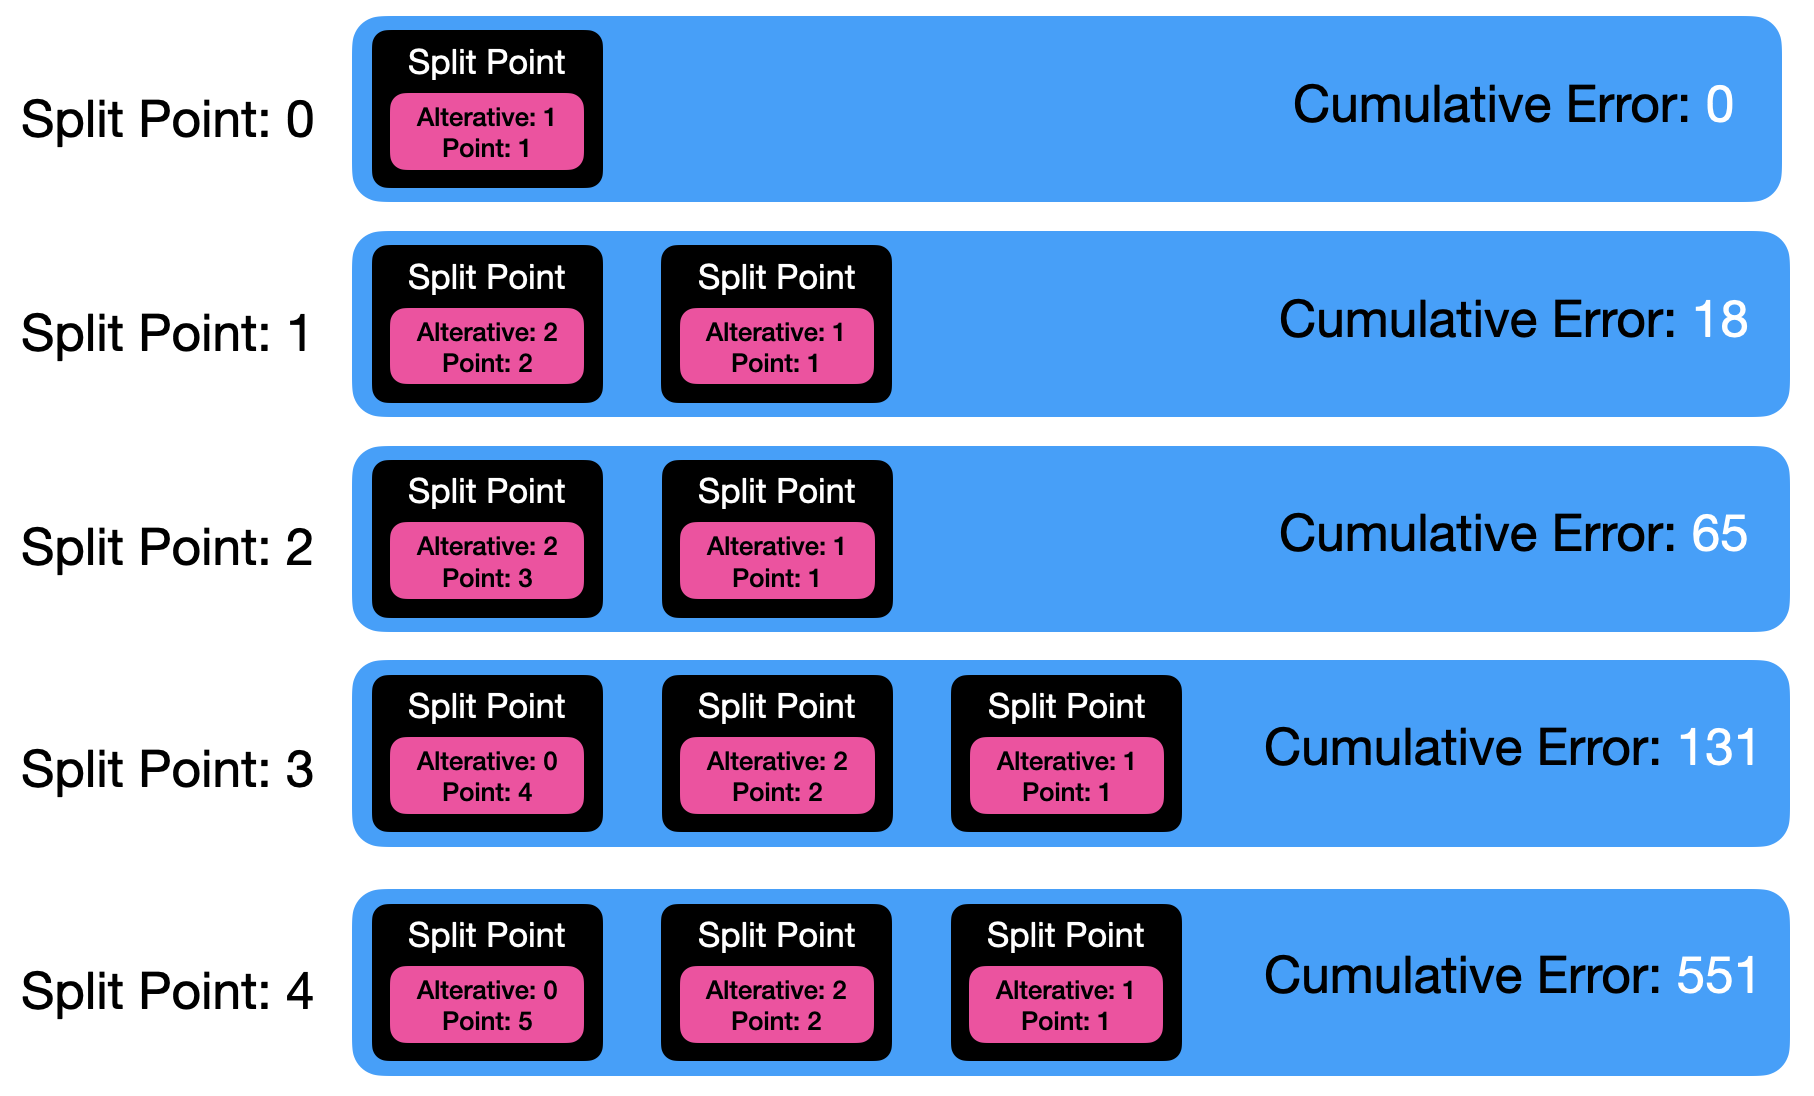
\includegraphics[scale=0.5]{candidate-list.png}
\caption{A visualization of the input to the "add split point" function.}
\label{fig:candidate-list}
\end{center}
\end{figure}

The last candidate in our list of candidates covers the entire range of 256 possible split points. The associated cumulative error has been minimized when no more changes can be made to any of the candidates. Because we repeatedly applied the “add split point” function until no more changes could be made, the algorithm has explored using all possible alternatives for all previous points and has converged on a decision of which split points were the best at each point. The last candidate’s list of split points leveraged all the knowledge explored by optimizing the candidates before it. Meaning we have found the optimal solution for the given set of alternatives. The list of possible split points associated with the final candidate is reversed and returned to the caller to generate a new alternative to be added to the set of possible alternatives of the original program.

\subsection{Why change the current algorithm?}


The regime phases of the compiler currently take up a sizable percentage of the Herbie nightly runs which are composed of 500+ benchmarks as seen in Figure \ref{fig:before-after}. This is used to get an aggregate of how Herbie is doing in its various phases and can be interpreted as how Herbie might perform for any arbitrary specification. With this insight, Herbie could spend a decent amount of time in the Regimes phase. Optimizing Regimes and improving the runtime has the benefit of lowering the potential time spent in the Regimes phase. Improving the runtime of the Regimes phase could surface other areas of Herbie that could benefit from performance optimizations.

The original dynamic algorithm leverages sub-problems and uses a basic level of memoization by precomputing the cumulative error sum for each alternative and using a recursive method of solving subproblems repeatedly until no more improvements can be made. This is already shown to terminate and provide a solution that meets the contract of providing a list of split points, that can be converted to an alternative program that has equal or less cumulative error than the alternatives it is composed of.

As discussed in section 6 of the “Algorithms Design” \cite{Algorithm} text cited in the Regimes sections of the Herbie paper, recursive solutions like this can often be reimplemented as iterative solutions over the subproblems. Moving to an approach like this has the potential to remove the recursive function calls and their associated cost while also reducing the amount of duplicate information being created and passed around between these function calls. 

Figure \ref{fig:candidate-list} displays how this list of subproblems is represented and shows that the best set of split points for a given point is directly represented as a Candidate with a list of split points saved at that point. This means that split points are copied between Candidates if they are used as part of a solution at a later point. When adding a new split point at any point during the algorithm, an allocation is made for this new list of split points each time a split point is added. This means the same split point is added to the data structure multiple times and is one area that could be improved on.

\subsection{The New Algorithm}

To preserve the contract of the original function that we are optimizing we need to construct a similar list of split points to return. The original algorithm also leverages memoization by saving results of smaller subproblems and builds up to the best solution from those sub-problems. We built up this list of split points by minimizing the error for each of the sub-problems. If at any point we found a better combination of alternatives to use up to a given point we constructed a new list of split points which indicates which alternative to use at any given point. This process requires three points of information to keep track of the cumulative error at each point, which alternative to use at a given point, and which point we previously split on before that point.

\begin{figure}[htbp]
\begin{center}
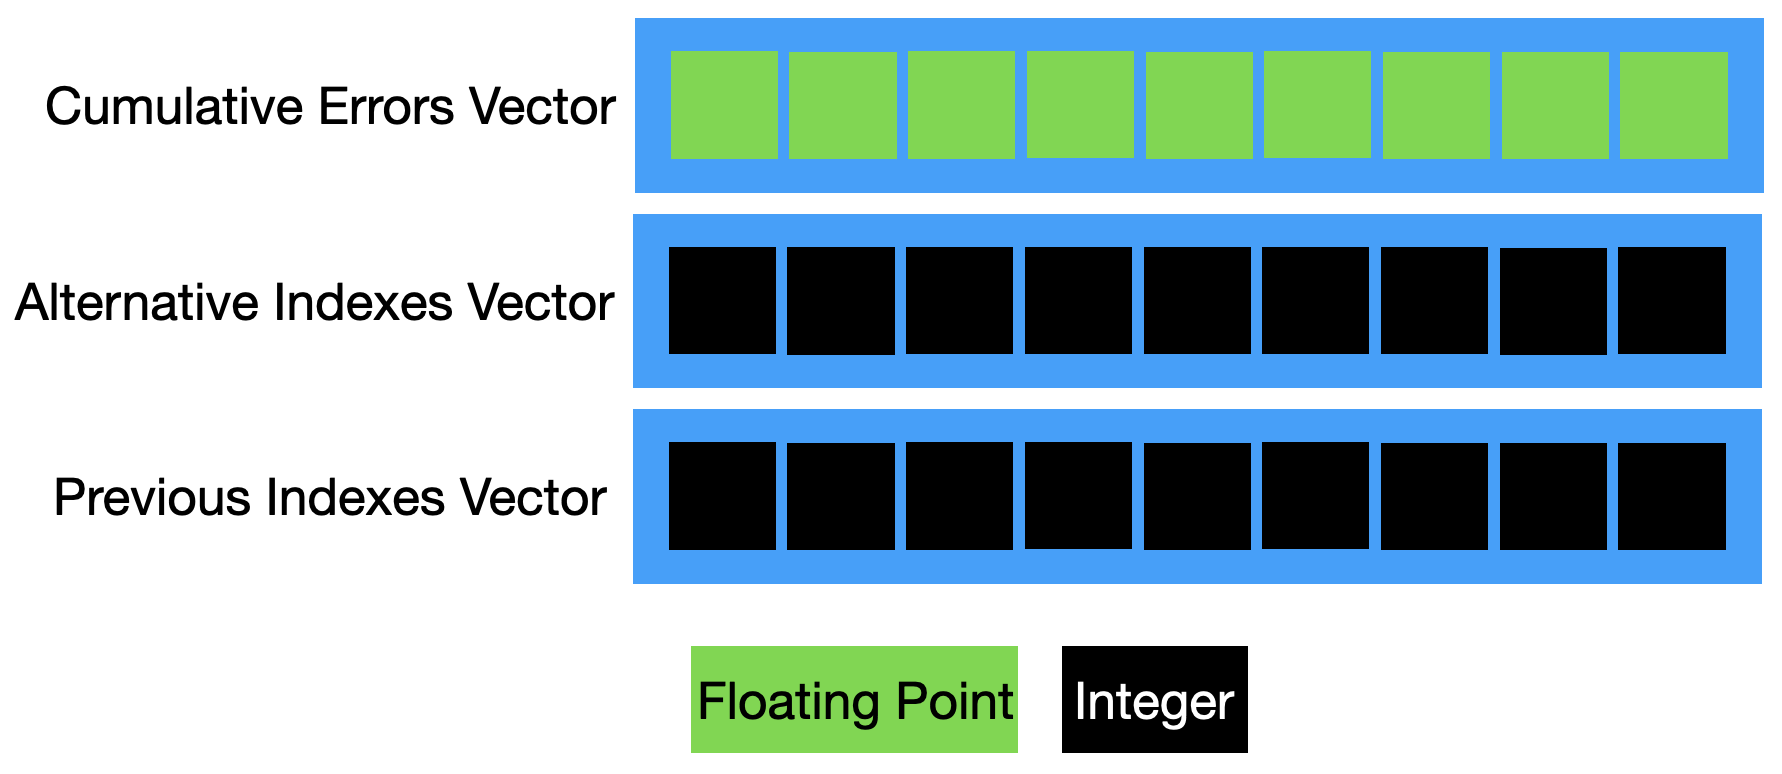
\includegraphics[scale=0.5]{vectors.png}
\caption{A visualization of the main data layout in the new algorithm.}
\label{fig:vectors}
\end{center}
\end{figure}

Instead of recursively nesting this information in a list of split points we can flatten this out into three vectors and keep track of each data point separately, as is shown in Figure \ref{fig:vectors}. The cumulative errors entry will represent the error up to that point. The alternative index indicates which alternative was used at that point and which difference in error was combined with a previous split point, if any. The Previous Indexes Vector stores indexes that represent the location of each of the possible previous split points that could be made.

These vectors are initially filled with infinity for the cumulative error, zero for the alternative index, and the Previous Indexes Vector is filled with the value of the total number of points. This previous index when not changed to another index in the vectors indicates not to use any additional split points.

To solve for the best set of split points as we did in the original algorithm we start by laying out an initial proposed solution, then iterate over each point as a subproblem to find the best solution for that point and update the data at that point if it beats the initial solution. This leaves behind the information needed to construct a list of split points with a similar result to the original algorithm.

We then generate an initial proposed solution by choosing the alternative with the lowest cumulative error at each point and save the cumulative error for that alternative at that point, along with which alternative it came from. This leaves the Previous Index Vector unmodified. We iterate over each possible split point (0 to 255) and solve for the best possible decision to make for that potential split point. When constructing the list of split points to return after finding the best decision for all possible split points, we loop over the points in reverse using the previous decisions of what split point is the best possible split point to be used at each point to generate a list of split points of which alternative should be used at which point and if additional split points are to be added. This approach explores all possible best-split points that could be made at each point but only uses the best solution found at the last point.

To compute the best decisions at each point we explore all previous points up to the current point. Calculating the delta error of each alternative between the current point and the point we are optimizing. This results in two temporary vectors, one of which alternative has the lowest increase in error and one with that delta of error between that point and the point we are optimizing. These two vectors are then looped over and the increased delta error is added to the cumulative error saved in our cumulative error vector. This gives a total error for the current point we are working on if we used that alternative combined with adding a split point at the previous point. Each of these totals is compared to the current cumulative error value at the current point. The current value is favored by adding our penalty value to the proposed total. If this weighted total is less than the current cumulative error, we update the cumulative error, the index of the alternative being used at that point, and the index of the previous cumulative error used for our new total. 

This process is repeated for all indexes 0 to 255 solving for the best possible decision that can be made at each point. When looping back over these arrays to construct our list of split points, if at any point we index into a point at which the Previous Index is still 256 we have found the last split point that can be created and can terminate and return our list of split points. This has allowed us to explore all possible points before the last point and make a decision on what the best set of splits is given the list of alternatives.

\section{Results}

This new approach has fewer runtime allocations since it is primarily computing the differences in error for each point and comparing combinations of alternatives at each point. This approach also slightly changes the order in which solutions are explored. Previously the order of exploration was the possible number of split points, per number of points, and per number of alternatives. In the new approach we explore over the number of points, the number of alternatives, and then the number of points. This is because there are big improvements to be made by pushing the alternatives to loop over all outermost loops. This new algorithm produces similar valid solutions but is about 3.5x faster and uses 7x less memory than the previous solution, as is shown in Figure \ref{fig:before-after}.


\begin{figure}[htbp]
\begin{center}
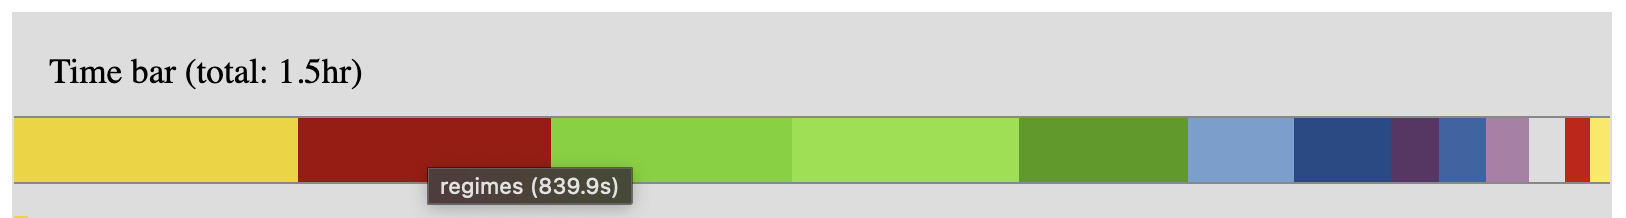
\includegraphics[width=0.95\textwidth]{regimes-before.png}
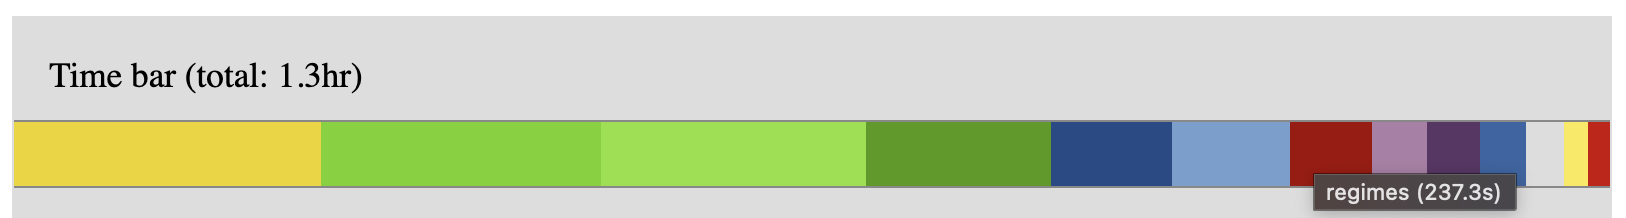
\includegraphics[width=0.95\textwidth]{regimes-after.png}
% TODO put memory usage side by side.

\includegraphics[width=0.80\textwidth]{memory-before.png}

\includegraphics[width=0.80\textwidth]{memory-after.png}
% TODO fix inconsistent memory image size
\caption{Before and after an aggregate of 500+ benchmark expressions.}
% Label is used to reference the image
\label{fig:before-after} 
\end{center}
\end{figure}

As you can see this moved regimes from being a large percentage of Herbie’s runtime down to being a much smaller part of the runtime. 


\subsection{Future Work}
Future work for regimes could include pushing the alternatives loop to the outermost loop. As this algorithm isn’t called just once it is called with a decreasing amount of alternatives, pruning alternatives with a higher average error on each call to Regimes. So pushing out the alternatives loop and exploring which alternative to use at each point has the added benefit of possibly compressing these outer calls into the Regimes algorithm and exploring all alternatives at once then looping over the resulting data and possibly generating multiple split points while only processing the alternatives once, saving work between these calls and reducing computations.

Another avenue of possible future improvements that could be made is tuning the penalty for when to add split points. A nice way of allowing for this would be surfacing this value as an input from a command line flag and later out to a more accessible front end like Odyssey. Allowing the client to experiment with different penalty values and see how that affects the number of branches added and the average error of an expression. Extending this idea allows for passing in a vector of weights for each possible split point representing a distribution of their inputs. For example, a program may have to accept inputs ranging from negative infinity to positive infinity, but maybe the program has heuristics that say 90\% of the inputs will be between -1 and 1. This distribution could be passed in as a vector of weights, and the cost of adding a given split point could vary based on this distribution. Having a higher penalty for a split inside the more concentrated area of inputs and a lower penalty for adding branches outside the first quantile. 


\section{Conclusion}

We flattened out a dynamic algorithm from refactoring a recursive solution to its iterative form. This reduces the redundant creation of information during the exploration of possibilities and favors computing the best possible solution at each point while only saving that information. This reduced the number of allocations needed to achieve the same output as the original algorithm. Overall we ended up making a 3.5x improvement in speed and a 7x reduction in memory usage, leading to a roughly 28\% speed up to the nightly benchmark suite, a small step for Herbie and a big step for Regimes.

\newpage
\bibliographystyle{plain}
\bibliography{citations}
\newpage
\appendix
% TODO Racket source code highlighter?
\lstset{style=racket-source-code}
\section{Regimes Old Algorithm}
Racket source code
\label{appendix:old-algorithm} 
\begin{lstlisting}
(define/contract (err-lsts->split-indices err-lsts can-split-lst)
  (->i ([e (listof list)] [cs (listof boolean?)]) 
        [result (cs) (curry valid-splitindices? cs)])
  (define num-candidates (length err-lsts))
  (define num-points (length (car err-lsts)))
  (define min-weight num-points)
  ; cumulative error sum
  (define psums (map (compose partial-sums list->vector) err-lsts))
  (define can-split? (curry vector-ref (list->vector can-split-lst)))
  
  (define initial
    (for/vector #:length num-points ([point-idx (in-range num-points)])
      (argmin cse-cost
              (map (λ (cand-idx cand-psums)
                     (let ([cost (vector-ref cand-psums point-idx)])
                       (cse cost (list (si cand-idx (+ point-idx 1))))))
                   (range num-candidates)
                   psums))))

  (define (add-splitpoint sp-prev)
    (for/vector #:length num-points
                ([point-idx (in-naturals)]
                 [point-entry (in-vector sp-prev)])
      (let ([acost (- (cse-cost point-entry) min-weight)]
            [aest point-entry])
        (for ([prev-split-idx (in-range 0 point-idx)]
              [prev-entry (in-vector sp-prev)]
              #:when (can-split? (si-pidx (car (cse-indices prev-entry)))))
          (let ([best #f] [bcost #f])
            (for ([cidx (in-naturals)] [psum (in-list psums)])
              (let ([cost (- (vector-ref psum point-idx) 
                             (vector-ref psum prev-split-idx))])
                (when (or (not best) (< cost bcost))
                  (set! bcost cost)
                  (set! best cidx))))
            (when (and (< (+ (cse-cost prev-entry) bcost) acost))
              (set! acost (+ (cse-cost prev-entry) bcost))
              (set! aest (cse acost (cons (si best (+ point-idx 1)) 
                                          (cse-indices prev-entry)))))))
        aest)))
  (define final
    (let loop ([prev initial])
      (let ([next (add-splitpoint prev)])
        (if (equal? prev next)
            next
            (loop next)))))
  (reverse (cse-indices (vector-ref final (- num-points 1)))))
\end{lstlisting}
\newpage
\section{Regimes New Algorithm}
Racket source code
\label{appendix:new-algorithm} 
\begin{lstlisting}
(define/contract (err-lsts->split-indices err-lsts can-split-lst)
  (->i ([e (listof list)] [cs (listof boolean?)]) 
        [result (cs) (curry valid-splitindices? cs)])
  (define can-split-vec (list->vector can-split))
  (define (make-vec-psum lst)
    (flvector-sums (list->flvector lst)))
  ; cumulative error sum
  (define flvec-psums (vector-map make-vec-psum (list->vector err-lsts)))
  (define number-of-points (vector-length can-split-vec))
  (define min-weight (fl number-of-points))
  
  (define result-error-sums (make-flvector number-of-points +inf.0))
  (define result-alt-idxs (make-vector number-of-points 0))
  (define result-prev-idxs (make-vector number-of-points number-of-points))
  
  (for ([alt-idx (in-naturals)]
        [alt-errors (in-vector flvec-psums)])
    (for ([point-idx (in-range number-of-points)]
          [err (in-flvector alt-errors)]
          #:when (< err (flvector-ref result-error-sums point-idx)))
      (flvector-set! result-error-sums point-idx err)
      (vector-set! result-alt-idxs point-idx alt-idx)))

  (define best-alt-idxs (make-vector number-of-points))
  (define best-alt-costs (make-flvector number-of-points))
  (for ([point-idx (in-range 0 number-of-points)]
        [current-alt-error (in-flvector result-error-sums)]
        [current-alt-idx (in-vector result-alt-idxs)]
        [current-prev-idx (in-vector result-prev-idxs)])
    (vector-fill! best-alt-idxs #f)
    (for ([point (in-range number-of-points)])
      (flvector-set! best-alt-costs point +inf.0))
    (for ([alt-idx (in-naturals)]
          [alt-error-sums (in-vector flvec-psums)])
      (for ([prev-split-idx (in-range 0 point-idx)]
            [prev-alt-error-sum (in-flvector alt-error-sums)]
            [best-alt-idx (in-vector best-alt-idxs)]
            [best-alt-cost (in-flvector best-alt-costs)]
            [can-split (in-vector can-split-vec 1)]
            #:when can-split)
        (let ([current-error (fl- (flvector-ref alt-error-sums point-idx) 
                                  prev-alt-error-sum)])
          (when (or (not best-alt-idx) (fl< current-error best-alt-cost))
            (flvector-set! best-alt-costs prev-split-idx current-error)
            (vector-set! best-alt-idxs prev-split-idx alt-idx)))))

    (for ([prev-split-idx (in-range 0 point-idx)]
          [r-error-sum (in-flvector result-error-sums)]
          [best-alt-idx (in-vector best-alt-idxs)]
          [best-alt-cost (in-flvector best-alt-costs)]
          [can-split (in-vector can-split-vec 1)]
          #:when can-split)
      (define set-cond
        (cond
          [(fl< alt-error-sum current-alt-error) #t]
          [(and (fl= alt-error-sum current-alt-error) 
                (> current-alt-idx best-alt-idx)) #t]
          [(and (fl= alt-error-sum current-alt-error)
                (= current-alt-idx best-alt-idx)
                (> current-prev-idx prev-split-idx)) #t]
          [else #f]))
      (when set-cond
        (set! current-alt-error alt-error-sum)
        (set! current-alt-idx best-alt-idx)
        (set! current-prev-idx prev-split-idx)))
    (flvector-set! result-error-sums point-idx current-alt-error)
    (vector-set! result-alt-idxs point-idx current-alt-idx)
    (vector-set! result-prev-idxs point-idx current-prev-idx))

  (define next number-of-points)
  (define split-idexs #f)
  (for ([i (in-range (- number-of-points 1) -1 -1)]
        #:when (= (+ i 1) next))
    (define alt-idx (vector-ref result-alt-idxs i))
    (define split-idx (vector-ref result-prev-idxs i))
    (set! next (+ split-idx 1))
    (set! split-idexs
          (cond
            [(false? split-idexs) (cons (si alt-idx number-of-points) '())]
            [else (cons (si alt-idx (+ i 1)) split-idexs)])))
  split-idexs)
\end{lstlisting}

\end{document}